%% Template file for all Software/Hardware modules

% Replace "Name of Module" with the name of this module
\chapter{Satellite Prototype}

\section{Description}

% Insert a description of the module here. This should include:
%  * The module's purpose
The purpose of the Satellite is to measure and transmit the voltage,
and the amount of current being drawn on the particular outlet that 
the Satellite is plugged into. The module is done this way so that
the current and voltage can be measured quickly and efficiently.
%  * Why the module is done this way

\section{Circuit Diagrams}

% This should consist of all the relevant circuit diagrams

Figure \ref{MeasuringCircuit} shows the layout of the Satellite's 
measuring hardware. Mains electricity will be run through a current
transformer which will measure only a fraction of the actual current. 
This will be enough to determine how much is actually being drawn. 
We then pass the current through a diode to ensure that it cannot 
reverse direction. The current will go through a resistor and 
then into an Analog to Digital converter.

\begin{figure}[H]
\centering
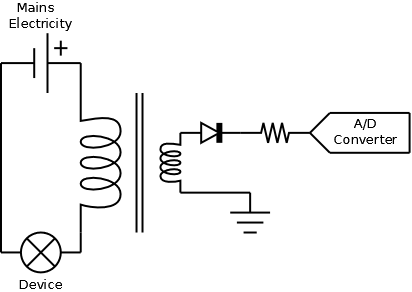
\includegraphics[scale=0.3]{Hardware/images/MeasureCircuit.png}
\caption{Measuring Circuit}
\label{MeasuringCircuit}
\end{figure}

\section{Potential Problems}

% A list of potentional programs along with suggestions
%  on ways to work around them. Elaborate on why the problem
%  exists

\section{Sub-modules 1}

% This is a second section of modules,
%  and should consists of this module broken 
%  down further into components. This would
%  be where you expand on any component of the circuit
%  if that needs to be done